\documentclass[a4paper, 12pt]{article}

\newcommand{\templates}{../../template}
\usepackage[a4paper, margin=2.5cm]{geometry}

\usepackage{enumitem}
\setlist[itemize]{noitemsep}
\setlist[enumerate]{noitemsep}

\let\oldpar\paragraph
\renewcommand{\paragraph}[1]{\oldpar{#1\\}\noindent}
\usepackage{graphicx}
\usepackage{hyperref}
\usepackage{makecell}

\newcommand{\settitolo}[1]{\newcommand{\titolo}{#1\\}}
\newcommand{\setprogetto}[1]{\newcommand{\progetto}{#1\\}}
\newcommand{\setcommittenti}[1]{\newcommand{\committenti}{#1\\}}
\newcommand{\setredattori}[1]{\newcommand{\redattori}{#1\\}}
\newcommand{\setrevisori}[1]{\newcommand{\revisori}{#1\\}}
\newcommand{\setresponsabili}[1]{\newcommand{\responsabili}{#1\\}}
\newcommand{\setversione}[1]{
	\ifdefined\versione\renewcommand{\versione}{#1\\}
	\else\newcommand{\versione}{#1\\}\fi
}
\newcommand{\setdestuso}[1]{\newcommand{\uso}{#1\\}}
\newcommand{\setdescrizione}[1]{\newcommand{\descrizione}{#1\\}}

\newcommand{\makefrontpage}{
	\begin{titlepage}
		\begin{center}

		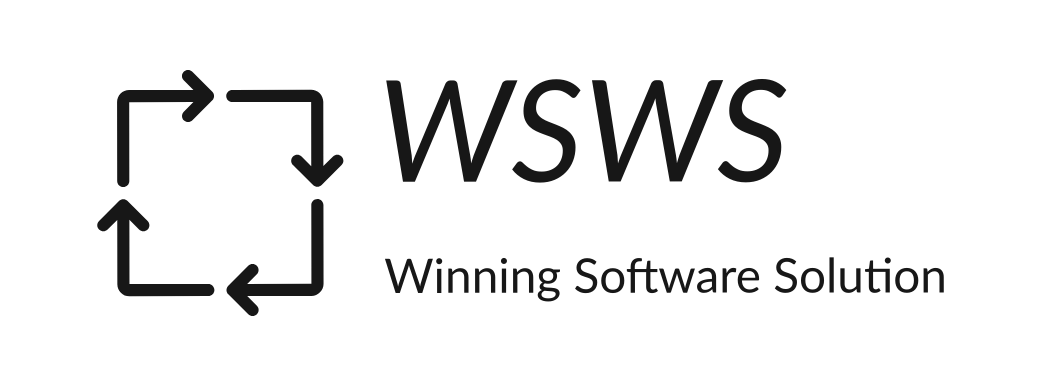
\includegraphics[width=0.4\textwidth]{../../template/WSWS-logos_transparent_crop}\\

		{\Large Winning Software Solution}\\[6pt]
		\href{mailto://winningsoftwaresolution@gmail.com}{winningsoftwaresolution@gmail.com}\\
		
		\ifdefined\progetto
		\vspace{1cm}
		{\Large\progetto}
		{\large\committenti}
		\else\fi
		
		\vspace{1.5cm}
		{\LARGE\titolo}
		
		\vfill
		
		\begin{tabular}{r | l}
		\multicolumn{2}{c}{\textit{Informazioni}}\\
		\hline
		
		\ifdefined\redattori
			\textit{Redattori} &
			\makecell[l]{\redattori}\\
		\else\fi
		\ifdefined\revisori
			\textit{Revisori} &
			\makecell[l]{\revisori}\\
		\else\fi
		\ifdefined\responsabili
			\textit{Respondabili} &
			\makecell[l]{\responsabili}\\
		\else\fi
		
		\ifdefined\versione
			\textit{Versione} & \versione
		\else\fi
		
		\textit{Uso} & \uso
		
		\end{tabular}
		
		\vspace{2cm}
		
		\ifdefined\descrizione
		Descrizione
		\vspace{6pt}
		\hrule
		\descrizione
		\else\fi
		\end{center}
	\end{titlepage}
}
\usepackage{hyperref}
\usepackage{array}
\usepackage{tabularx}

\def\vers#1-#2-#3-#4-#5\\{#1&#2&#3&#4&#5\\\hline}

\newcommand{\addversione}[5]{
	\ifdefined\versioni
		\let\old\versioni
		\renewcommand{\versioni}{#1&#2&#3&#4&#5\\\hline\old}
	\else
		\newcommand{\versioni}{#1&#2&#3&#4&#5\\\hline}
	\fi
}

\newcommand{\setversioni}[1]{\newcommand{\versioni}{#1}}

\newcommand{\makeversioni}{
	\begin{center}
		\begin{tabularx}{\textwidth}{|c|c|c|c|X|}
		\hline
		\textbf{Versione} & \textbf{Data} & \textbf{Persona} & \textbf{Attivtà} & \textbf{Descrizione} \\
		\hline
		\versioni
		\end{tabularx}
	\end{center}
	\clearpage
}
\usepackage{hyperref}
\usepackage{graphicx}
\usepackage{placeins}
\settitolo{Manuale E-commerce Shop Chain}
\setredattori{WinningSoftwareSolution}
\setdestuso{esterno}
\setdescrizione{
Manuale e-commerce.
}

\begin{document}

\makefrontpage
\tableofcontents
\newpage

\section{Introduzione}
Attraverso l'utilizzo della blockchain \textit{Polygon}, Shop Chain fornisce un sistema decentralizzato per il pagamento di prodotti in MATIC. Utilizzando Shop Chain è possibile effettuare una qualsiasi attività di compravendita in maniera sicura per entrambi gli attori dello scambio. L'acquirente che desidera acquistare un prodotto da un venditore in un e-commerce potrà effettuare il suo pagamento in MATIC, ovvero il token nativo della blockchain \textit{Polygon}. Il venditore non può disporre immediatamente del saldo ricevuto poiché sarà bloccato fino alla ricezione del pacco, momento nel quale l'acquirente può sbloccare i fondi attraverso la scannerizzazione di un codice QR presente sulla scatola.
Il presente documento ha la funzione di descrivere in dettaglio la procedura da seguire per l'e-commerce al fine di vendere correttamente i propri prodotti.

\section{Vendita di prodotti}
\subsection{Wallet Metamask}
Per poter vendere i propri prodotti sarà necessario utilizzare un wallet Metamask. Visitare \href{https://www.metamask.io}{metamask.io} per maggiori informazioni.
\subsubsection{Configurazione}
Se il network \textit{Polygon} non è gia stato inserito nel proprio wallet Metamask, procedere con la lettura del seguente paragrafo.
Per l'inserimento e la configurazione del network \textit{Polygon} nel proprio wallet Metamask è necessario utilizzare i seguenti dati:
\begin{itemize}
\item Network Name: \textbf{Matic Mainnet};
\item New RPC Url: \textbf{https://rpc-mainnet.maticvigil.com/};
\item ChainID: \textbf{137};
\item Currency Simbol: \textbf{MATIC};
\item Block Explorer URL: \textbf{https://explorer.matic.network/}.
\end{itemize}
Una volta inseriti i dati e aggiunto il network, ricordare di selezionare il network.

\subsubsection{Collegamento del wallet a Shop Chain}
Una volta inserito correttamente il network è necessario collegare il proprio wallet metamask a Shop Chain. Una volta reindirizzati sulla landing page di Shop Chain, se non si ha già collegato in precedenza il proprio wallet:
\begin {itemize}
\item selezionare "Connect Wallet" all'apertura del pop-up (Fig. 1);
\item approvare il collegamento dal proprio wallet Metamask.
\end{itemize}

\FloatBarrier
\begin{figure}
\centering
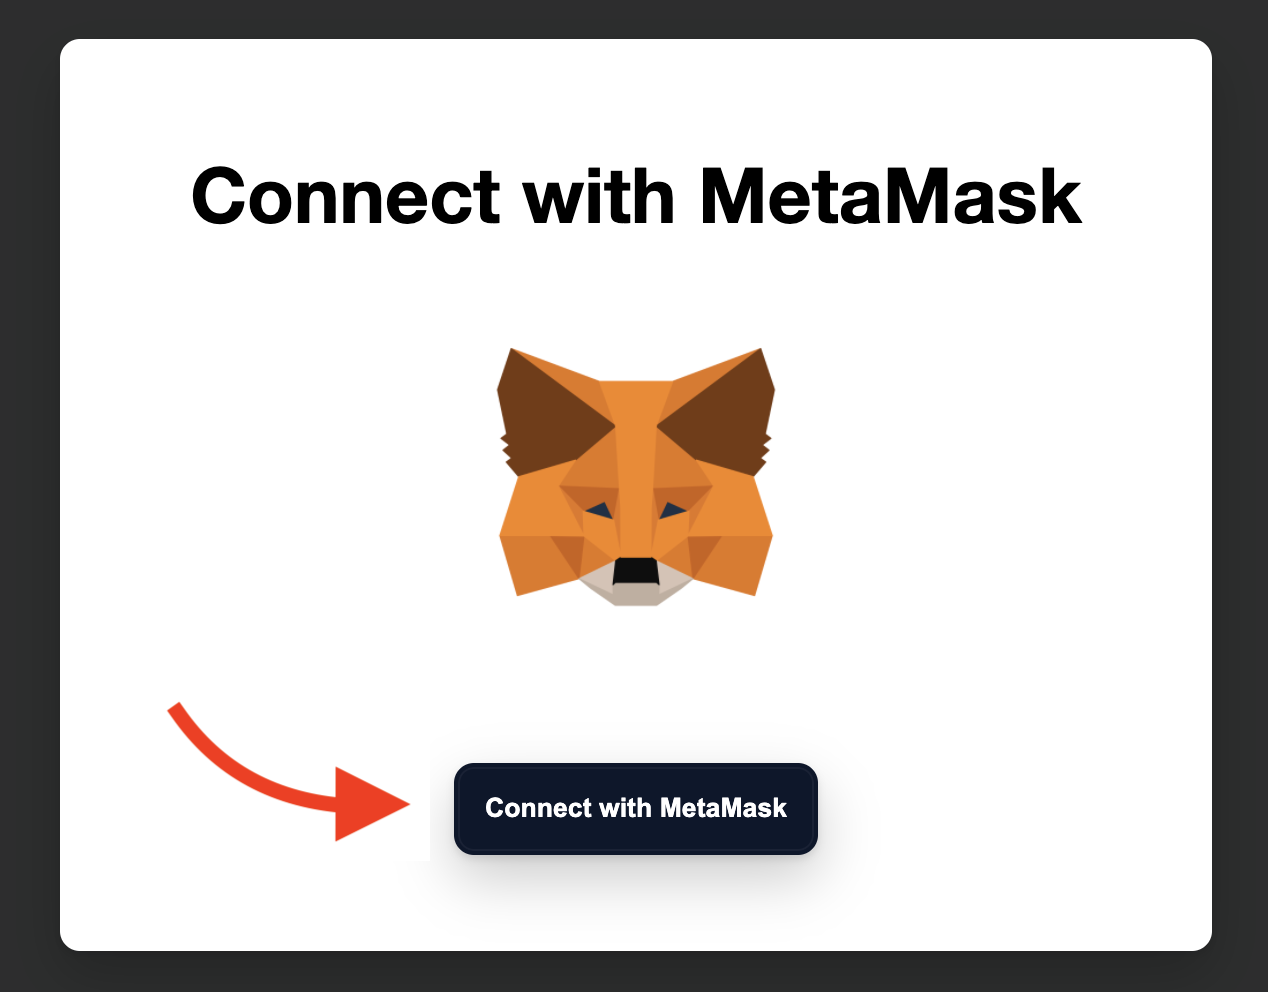
\includegraphics[width=0.5\linewidth]{img/connessione_wallet.png}
\caption{Interfaccia per la connessione del wallet Metamask.}
\end{figure}
\FloatBarrier



\end{document}
